\documentclass[12pt]{book}
\usepackage{amsmath}
\usepackage{amsthm}
\usepackage{amssymb}
\usepackage{fontspec}
\usepackage{ctex}
\usepackage{graphicx}%\begin{figure}[H]\centering\includegraphics[width=1\textwidth]{}\end{figure}
\usepackage{xcolor}
\usepackage{stmaryrd}%输入特定数学符号的宏包,如整数区间符号
\usepackage{wrapfig}%图文混排%\begin{wrapfigure}[10]{r}{2.3cm}\includegraphics[scale=0.5]{}\end{wrapfigure}
\usepackage{caption}%浮动体的标题
\usepackage{subfig}%排列多张图片
\usepackage{float}%[H]参数防止图片浮动到下一页
\usepackage{hyperref}
\theoremstyle{definition}\newtheorem{dfn}{Définition}[chapter]
\theoremstyle{plain}\newtheorem{thm}{Théorème}[chapter]
\theoremstyle{plain}\newtheorem{prp}{Proposition}[chapter]
\theoremstyle{plain}\newtheorem{lem}{\bf Lemme}[chapter]
\theoremstyle{plain}\newtheorem{axm}{\bf Axiome}[chapter]
\theoremstyle{plain}\newtheorem{lmm}{\bf Lemme}[chapter]
\theoremstyle{plain}\newtheorem{cor}{\bf Corollaire}[chapter]
\theoremstyle{remark}\newtheorem{rem}{Remarque}[chapter]
\title{Notes of maths}
\author{PhilippeMENG}
\date{\today}
\begin{document}
\maketitle
\tableofcontents
\frontmatter
这本书的出发点是我决心编写一本自己的数学百科全书。从我自己学习的角度,我非常需要一本自己的宝典来吸收百家之长,这是我能够不断阅读并取得真正效果保障。
\mainmatter

        \chapter{Vocabulaire de théorie des ensembles}

\begin{thm}[The Knaster-Tarski fixed-point theorem]
 Suppose that $A$ is a set and that $f: P(A) \rightarrow P(A)$ is an increasing function; if $B \subseteq C \subseteq A$ then $f(B) \subseteq f(C) .$ Then there exists $G \subseteq A$ such that $f(G)=G$.
\end{thm}

\begin{proof}
	Note that $f$ is defined as a mapping from $P(A)$ to itself: it is not defined in terms of a mapping from $A$ to itself. Thus $\emptyset \subseteq f(\emptyset)$ and $A \supseteq f(A) ;$ the inclusions change direction. The theorem states that equality holds at some intermediate subset.
	
	We shall show that there exists a set $G$ such that $G \subseteq f(G)$ and $f(G) \subseteq G$; the axiom of extensionality then ensures that $G=f(G)$. Let $\mathcal{G}=\{B \in P(A): B \subseteq f(B)\},$ and let $G=\cup_{B \in \mathcal{G}} B .$ If $B \in \mathcal{G}$
	then $B \subseteq G,$ and so $f(B) \subseteq f(G) .$ Thus $B \subseteq f(B) \subseteq f(G) .$ Consequently $G=\cup_{B \in \mathcal{G}} B \subseteq f(G),$ and so $G \in \mathcal{G} .$ On the other hand, since $G \subseteq f(G)$
	it follows that $f(G) \subseteq f(f(G)),$ and so $f(G) \in \mathcal{G} .$ Thus $f(G) \subseteq \cup_{B \in \mathcal{G}} B=$
	$G$

\end{proof}









We aim to show that if there are injections $f: A \rightarrow B$ and
$g: B \rightarrow A,$ then there is a bijection $h: A \rightarrow B .$
The proof of this fact, though not particularly difficult, is not
entirely trivial, either. The fact that $f$ and g guarantee that such
an $h$ exists is called the the {\bf Cantor-Bernstein-Schröeder theorem}. This theorem is very useful for proving two sets $A$ and $B$ have the same cardinality: it says that instead of finding a bijection $A \rightarrow B,$ it suffices to find injections $A \rightarrow B$ and $B \rightarrow A$. This is useful because injections are often easier to find than bijections.

We will prove the Cantor-Bernstein-Schröeder theorem, but before doing so let's work through an informal visual argument that will guide us through (and illustrate) the proof.

Suppose there are injections $f: A \rightarrow B$ and $g: B
\rightarrow A$. We want to use them to produce a bijection $h: A
\rightarrow B .$ Sets $A$ and $B$ are sketched below. For clarity,
each has the shape of the letter that denotes it, and to help
distinguish them the set $A$ is shaded.
\begin{figure}[H]\centering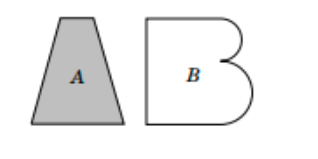
\includegraphics[width=0.6\textwidth]{image//Vocabulaire de theorie des ensembles//1}\end{figure}
The injections $f: A \rightarrow B$ and $g: B \rightarrow A$ are
illustrated in Figure  Think of $f$ as putting a "copy" $f(A)=\{f(x):
x \in A\}$ of $A$ into $B,$ as illustrated. This copy, the range of
$f,$ does not fill up all of $B$ (unless $f$ happens to be
surjective). Likewise, $g$ puts a "copy" $g(B)$ of $B$ into
$A$. Because they are not necessarily bijective, neither $f$ nor $g$
is guaranteed to have an inverse. But the map $g: B \rightarrow g(B)$
from $B$ to $g(B)=\{g(x): x \in B\}$ is bijective, so there is an
inverse $g^{-1}: g(B) \rightarrow B$. (We will need this inverse
soon.)
\begin{figure}[H]\centering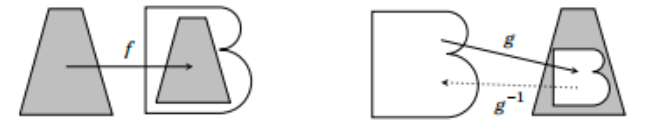
\includegraphics[width=1\textwidth]{image//Vocabulaire de theorie des ensembles//2}\end{figure}
Consider the chain of injections illustrated in the figure below.
\begin{figure}[H]\centering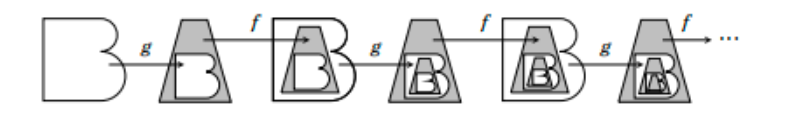
\includegraphics[width=1.2\textwidth]{image//Vocabulaire de theorie des ensembles//3}\end{figure}
 On the left, $g$ puts a copy of $B$ into $A$. Then $f$ puts a copy of $A$ (containing the copy of B) into $B$. Next, $g$ puts a copy of this $B$ -containing- $A$ -containing- $B$ into $A$, and so on, always alternating $g$ and $f$.

The first time $A$ occurs in this sequence, it has a shaded region $A-g(B) .$ In the second occurrence of $A$, the shaded region is $(A-g(B)) \cup(g \circ f)(A-g(B))$. In the third occurrence of $A$, the shaded region is
$$
(A-g(B)) \cup(g \circ f)(A-g(B)) \cup(g \circ f \circ g \circ f)(A-g(B))
$$

To tame the notation, let's say $(g \circ f)^{2}=(g \circ f) \circ(g \circ f)$, and $(g \circ f)^{3}=(g \circ f) \circ(g \circ f) \circ(g \circ f)$, and so on.Let's also agree that $(g \circ f)^{0}=I_{A}$, that is, it is the identity function on $\mathrm{A}$. Then the shaded region of the $n^{th}$ occurrence of $\mathrm{A}$ in the sequence is
$\bigcup\limits_{k=0}^{n-1}(g \circ f)^{k}(A-g(B))$
This process divides A into gray and white regions: the gray region is
$G=\bigcup\limits_{k=0}^{n-1}(g \circ f)^{k}(A-g(B))$
and the white region is $A-G$.
\begin{figure}[H]\centering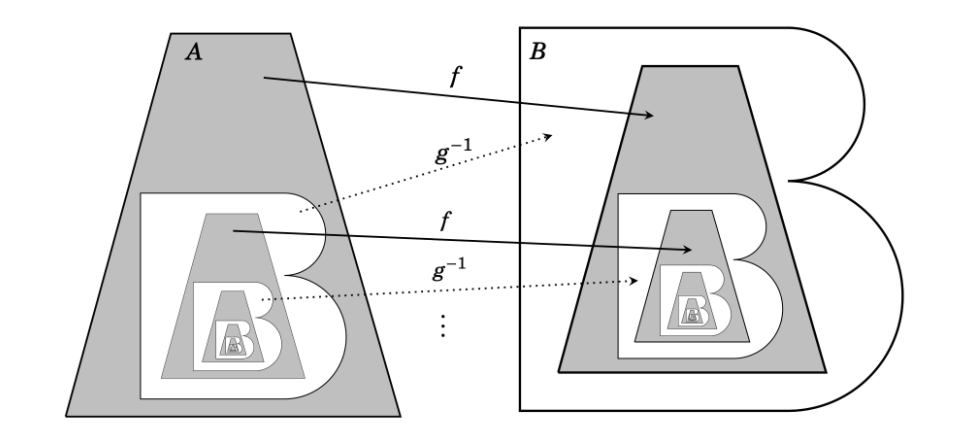
\includegraphics[width=1.2\textwidth]{image//Vocabulaire de theorie des ensembles//4}\end{figure}
The figure suggests our desired bijection $h: A \rightarrow B$. The
injection $f$ sends the gray areas on the left bijectively to the gray
areas on the right. The injection $g^{-1}: g(B) \rightarrow B$ sends
the white areas on the left bijectively to the white areas on the
right. We can thus define $h: A \rightarrow B$ so that $h(x)=f(x)$ if
$x$ is a gray point, and $h(x)=g^{-1}(x)$ if $x$ is a white point.
This informal argument suggests that given injections $f: A \rightarrow B$ and $g: B \rightarrow A$, there is a bijection $h: A \rightarrow B$. But it is not a proof. We now present this as a theorem and tighten up our reasoning in a careful proof, with the above diagrams and ideas as a guide.
\begin{thm}[The Cantor-Bernstein-Schroder Theorem]
If $|A| \leq|B|$ and $|B| \leq|A|,$ then $|A|=|B| .$ In other words, if there are injections $f: A \rightarrow B$ and $g: B \rightarrow A,$ then there is a bijection $h: A \rightarrow B$.
\end{thm}
 \begin{proof}
({\bf Direct})

Suppose there are injections $f: A \rightarrow B$ and $g: B \rightarrow A$. Then, in particular, $g: B \rightarrow g(B)$ is a bijection from B onto the range of $g,$ so it has an inverse $g^{-1}: g(B) \rightarrow B$. (Note that $g: B \rightarrow A$ itself has no inverse $g^{-1}: A \rightarrow B$ unless $g$ is surjective.)

Consider the subset $G=\bigcup\limits_{k=0}^{n-1}(g \circ f)^{k}(A-g(B)) \subseteq A$
Let $W=A-G$, so $A=G \cup W$ is partitioned into two sets G (think gray) and W (think white). Define a function $h: A \rightarrow B$ as
$h(x)=\left\{\begin{array}{cl}f(x) & \text { if } x \in G \\ g^{-1}(x) & \text { if } x \in W\end{array}\right.$
Notice that this makes sense: if $x \in W,$ then $x \notin G,$ so $x \notin A-g(B) \subseteq G,$ hence $x \in g(B),$ so $g^{-1}(x)$ is defined.

To finish the proof, we must show that $\mathrm{h}$ is both injective and surjective.

For injective, we assume $h(x)=h(y),$ and deduce $x=y .$ There are three cases to consider. First, if $x$ and $y$ are both in $G,$ then $h(x)=h(y)$ means $f(x)=f(y),$ so $x=y$ because $f$ is injective. Second, if $x$ and $y$ are both in $W,$ then $h(x)=h(y)$ means $g^{-1}(x)=g^{-1}(y),$ and applying $g$ to both sides gives $x=y$. In the third case, one of $x$ and $y$ is in $G$ and the other is in $W$. Say $x \in G$ and $y \in W$. The definition of G gives $x=(g \circ f)^{k}(z)$ for some $k \geq 0$ and $z$ in $A-g(B)$. Note $h(x)=h(y)$ now implies $f(x)=g^{-1}(y),$ that is, $f\left((g \circ f)^{k}(z)\right)=g^{-1}(y)$. Applying $g$ to both sides gives $(g \circ f)^{k+1}(z)=y,$ which means $y \in G .$ But this is impossible, as $y \in W$. Thus this third case cannot happen. But in the first two cases $h(x)=h(y)$ implies $x=y,$ so $h$ is injective.

To see that $h$ is surjective, take any $b \in B$. We will find an $x \in A$ with $h(x)=b$. Note that $g(b) \in A,$ so either $g(b) \in W$ or $g(b) \in G$. In the first case, $h(g(b))=g^{-1}(g(b))=b,$ so we have an $x=g(b) \in A$ for which $h(x)=b$. In the second case, $g(b) \in G .$ The definition of G shows $g(b)=(g \circ f)^{k}(z)$
for some $z \in A-g(B)$ and $k \geq 0$. In fact we have $k>0,$ because $k=0$ would give $g(b)=(g \circ f)^{0}(z)=z \in A-g(B),$ but clearly $g(b) \notin A-g(B)$. Thus $g(b)=(g \circ f) \circ(g \circ f)^{k-1}(z)=g\left(f\left((g \circ f)^{k-1}(z)\right)\right) .$ Because $g$ is injective, this implies $b=f\left((g \circ f)^{k-1}(z)\right).$Let $x=(g \circ f)^{k-1}(z),$ so $x \in G$ by definition of $G$. Observe that $h(x)=f(x)=f\left((g \circ f)^{k-1}(z)\right)=b$. We have now seen that for any $b \in B$, there is an $x \in A$ for which $h(x)=b$. Thus $h$ is surjective.

Since $h: A \rightarrow B$ is both injective and surjective, it is also bijective.

 \end{proof} 
\begin{proof}
({\bf Indirect})

The existence of $f$ says that ' $A$ is no bigger than $B$ ' and the existence of $g$ says that ' $B$ is no bigger than $A$ '. The conclusion then is that if both hold then ' $A$ and $B$ are the same size'. We shall consider the problem of whether two sets are always comparable in size later.

We consider the mappings $f: P(A) \rightarrow P(B)$ and $g: P(B) \rightarrow P(A)$ determined by $f$ and $g$; they are clearly increasing maps. On the other hand the mapping $C_{A}: P(A) \rightarrow P(A)$ defined by $C_{A}(D)=A \backslash D$ is order reversing, as is the corresponding mapping $C_{B}: P(B) \rightarrow P(B)$. Thus the composite mapping $S=C_{A} \circ g \circ C_{B} \circ f$ is an increasing mapping from $P(A)$ into itself. The Knaster-Tarski fixed-point theorem then tells us that there exists $D \subseteq A$ such that $S(D)=D ;$ the restriction $f_{\mid D}$ of $f$ to $D$ is a bijection of $D$ onto $f(D) .$ Let $E=f(D),$ so that $C_{B}(f(D))=B \backslash E .$ Thus
$$
\begin{aligned}
A \backslash D &=C_{A}(D)=C_{A}(S(D))=C_{A}\left(C_{A} g C_{B} f(D)\right) \\
&\left.=g\left(C_{B} f(D)\right)\right)=g(B \backslash E)
\end{aligned}
$$
Consequently the restriction $g_{\mid B \backslash E}$ of $g$ to $B \backslash E$ is a bijection of $B \backslash E$ onto $A \backslash D ;$ let $k: A \backslash D \rightarrow B \backslash E$ be its inverse. We now set $h(a)=f_{\mid D}(a)$
for $a \in D,$ and set $h(a)=k(a)$ for $a \in A \backslash D ; h$ clearly has the required properties.

\end{proof}










        \chapter{Logarithme}
        \paragraph{Propriété fondamentale} Une fonction continue strictement monotone sur un intervalle est une bijection de cet intervalle sur son image.


        \paragraph{Exposant rationnel}
        Soit $q\in \mathbb{N*}$.Alors,il est clair que la fonction $\varphi:\mathbb{R_+}\longrightarrow \mathbb{R},\quad x\longmapsto \sqrt[q]{x} $  est continue et strictement croissante.






        \chapter{Vector calculus}
        \section{The vector product(Axial vector)}
        \subsection{Rules of calculation}
        \paragraph{No associativity}
        \textbf{(a$\times$b)$\times$ c $\neq$ a$\times$(b$\times$ c)
        }     The vector on the left side lies in the plane spanned by the vectors \textbf{a} and \textbf{b} (因为the plane spanned by the vectors \textbf{a} and \textbf{b}和 The vector on the left side都与$\mathbf{a}\times\mathbf{b}$垂直) ; the vector on the right side is in the plane spanned by \textbf{b} and \textbf{c}. The subsequent example also shows that associativity does not hold. One has {$\mathbf{e_1}\times( \mathbf{e_2}\times \mathbf{e_2}) =\mathbf{0}$}, but {$(\mathbf{e_1}\times \mathbf{e_2})\times \mathbf{e_2} =\mathbf{-e_1}$}.






\chapter{The natural numbers}
\section{The Peano axioms}

To define the natural numbers,we will use two fundamental concepts: the zero number 0, and the increment operation.



\chapter{Ensembles des nombres réels}
\section{Densité de $\mathbb{Q}$ et de $\mathbb{R\setminus Q}$}
\begin{dfn}
        On dit que'une partie $A\subset \mathbb{R}$ est dense dans $\mathbb{R}$ si :
        $$
        \forall a,b\in \mathbb{R},
        (a<b \Rightarrow A\cap ] a,b [\not=\emptyset )
        $$

\end{dfn}

\begin{prp}{\textbf{caractérisation séquentielle de la densité}}

        Soit A une partie de $\mathbb{R}$, A est dense dans $\mathbb{R}$ ssi pour
        tout $x \in \mathbb{R}$, il existe $(a_n)\in A^{\mathbb{N}}$ une suite d'élément de $A$ qui converge vers x.
\end{prp}

\section{Borne supérieure et borne inférieure}
\begin{dfn}
Soit $(E,\le)$ un ensemble ordonne,A une partie de E.
\begin{itemize}
        \item On dit que A admet une borne supérieure (dans E) si l'ensemble des majorants de A admet un plus petit élément.

        Dans ce cas,ce plus petit élément est appelé la borne supérieure de A et
        est noté $\sup A$
        $$
        \sup A=\min\{M\in E, M \quad majore\quad A\}=\min\{ M\in E  | \forall a\in A ,a\le M\}
        $$

        \item On dit que A admet une borne inférieure (dans E) si l'ensemble des minorants de A admet un plus grand élément.

        Dans ce cas,ce plus grand élément est appelé la borne inférieure de A et
        est noté $\inf A$
                $$
        \inf A=\max\{m\in E, m\text{ minore }A\}=\max\{ m\in E  | \forall a\in A ,m\le a\}
        $$


\end{itemize}
\end{dfn}

\begin{rem}
\textbf{注意sup与max的区别}
\begin{itemize}
\item si A admet un plus grand élément, alors $\max A=\sup A$.
\item Par contre la réciproque est fausse.Par exemple,$[0,1[$ admet une borne supérieure qui est 1 mais pas de plus grand élément
\end{itemize}
\end{rem}



\chapter{Généralités sur les fonctions d'une variable réelle}


\section{Fonctions lipschitziennes}



\begin{dfn}
Soient $f : I \rightarrow \mathbb{K}$ une fonction et $k \in \mathbb{R_{+}^{*}}$. On dit que f est k-lipschitzienne si :
$$\forall x,y \in I ,\left |   f(y)- f(x)\right | \le k \left |   y- x\right |
$$
\begin{itemize}

\item On dit qu'une fonction f est lipschitzienne s'il existe $k > 0$ tel que f soit k-lipschitzienne.
\item Si f est k-lipschitzienne avec $0 < k < 1$, on dit que f est k-{\color{red}contractante}.

\end{itemize}


\end{dfn}

\begin{rem}
La fonction cosinus est 1-lipschitzienne. En effet, soient x et y deux réels, alors :
$$
\begin{aligned}
\left|   \cos(y)-\cos(x)   \right| &=\left|\int_{x}^{y}\cos'(t)\mathrm{d}t \right|\\
&=\left|\int_{x}^{y}-\sin(t)\mathrm{d}t \right|\\
&\le\int_{I}\left|sin(t)\right|\mathrm{d}t&\text{où I = $\left[x, y\right]$ si x $\le$ y et I = $\left[y, x\right]$ sinon}\\
&\le\int_{I}\mathrm{d}t\\
&=\left| y-x \right|\\
\end{aligned}
$$
\end{rem}

\section{Fonctions monotones}

\begin{prp}
Soient $f : I\rightarrow R$ et$ g : J \rightarrow R$ deux applications. On suppose que :
\begin{itemize}
\item f et g sont monotones sur I et J respectivement ;

\item on peut définir la composée $g\circ f$, c'est-à-dire $f(I) \subset J$.
\end{itemize}

Alors la fonction $g\circ f$ est monotone sur I, la monotonie étant donné par \textbf{'la règle des signes'} (croissante : $+$ ,
décroissante : $-$). Autrement dit, si f et g sont de même monotonie, alors $g\circ f$ est croissante et si f et g sont de monotonies opposées, alors  $g\circ f$ est décroissante.
Par ailleurs, si f et g sont strictement monotones, alors  $g\circ f$ l'est aussi.

\end{prp}

\chapter{Étude locale d'une fonction}
\textbf{Cadre} Dans toute la suite, on se restreint à des fonctions définies sur un intervalle réel $I$ ayant au moins deux points, c'est-à-dire tel que $-\infty\le \inf I < \sup I\le \infty$.

On définie alor:
\begin{itemize}
\item L'intérieur de $I$, noté $\mathring{I}=]\inf I,\sup I[$.On a donc dans notre cadre $\mathring{I}\not = \emptyset$
\item L'adhérence de I,notée $\overline{I}$, par $\overline{I}=[\inf I,\sup I]\subset \overline{\mathbb{R}}.$
\end{itemize}
有必要强调,这里用inf和sup来定义区间形态实在比较易混淆,且$I$本身的状态不明确,有时用 $\mathring{I}$和$\overline{I}$只是起到一个确定强调的作用,并不代表$I$需要这么限制或衍生。但是这个I的框架是非常全面的,为了这个全面性,人为地增加了一点抽象度。
\begin{dfn}{\textbf{Voisinage d'un point}}

Soit $a\in \mathbb{R}$.On définit:
\begin{itemize}
        \item  la boule ouverte(respectivement fermée) de centre $a$ et de rayon $\alpha >0$ par $
        B(a,\alpha)=\left\{x\in \mathbb{R},|x-a|< \alpha\right\}$(respectivement $
        B_f(a,\alpha)=\left\{x\in \mathbb{R},|x-a|\le \alpha\right\}$).

        Les ensembles  $
        B(a,\alpha)$ pour $\alpha>0$ sont appelés des voisinages ouverts de $a$ (dans $\mathbb{R}$) et les ensembles $	B_f(a,\alpha)$ sont appelés des voisinages fermés de $a$ (dans $\mathbb{R}$);
        \item un voisinage ouvert (respectivement fermé)
        de $+\infty$ est un intervalle de la forme $]A,+\infty[$(respectivement $[A,+\infty[$) avec $A\in \mathbb{R}$;
                \item un voisinage ouvert (respectivement fermé)
        de $-\infty$ est un intervalle de la forme $]-\infty,A[$(respectivement $]-\infty,A]$) avec $A\in \mathbb{R}$.

\end{itemize}
\textbf{On note $\mathcal{V}_f(a)$ l'ensemble des voisinages fermés de $a$}.
\end{dfn}
值得注意的是,在$a$有限的情况下我们的领域实际上就是boule。另外,$\mathcal{V}_f(a)$是一个邻域的集合,里面的元素不是$x$,而是作为$x$的集合的闭邻域。
\begin{prp}
        $$
        a\in \overline{I}\ \Leftrightarrow \forall V\in \mathcal{V}_f(a),I\cap V\not =\emptyset.
        $$
\end{prp}
\begin{dfn}
Soit $f : I\rightarrow \mathbb{K}$ et $a \in \overline{I}$. On dit qu'une propriété relative à f est vraie au voisinage de a (ou localement en a) s'il existe un voisinage \textbf{ouvert} $\mathcal{B}$ de a telle que la propriété est vraie sur $I \cap \mathcal{B}$.
\end{dfn}

\begin{dfn}{Définition générale de la limite}
        Soient $a\in \overline{I},l\in \overline{\mathbb{R}}$ et $f:I\rightarrow \mathbb{R}.$ On dit que $f$ admet $l$ pour limite en $a$ si:
                $$
                \forall U\in \mathcal{V}_{f}(l),\exists V\in
                \mathcal{V}_{f}(a), \forall x\in I\cap V, f(x)\in U.
                $$
\end{dfn}

\begin{prp}{Limite d'une fonction composée et caractérisation séquentielle de la limite}
Soient $f:I\rightarrow J\subset \mathbb{R}$ et $g:J\rightarrow\mathbb{K}$ deux fonctions, a$\in \overline{I}$.On suppose que :

\begin{itemize}
\item[1.] $\lim_{x\to a}f(x)=l\in \overline{\mathbb{R}};$
\item[2.] $\lim_{x\to l}g(x)=L.$
\end{itemize}

Alors $g\circ f$ admet une limite en $a$ et $\lim_{x\to a}(g\circ f)(x)=L.$

\end{prp}

\chapter{Relation de comparaisons}
\begin{prp}
$f\underset{a}{=}o(g)$ si et seulement si il existe une fonction $h$, définie sur un voisinage $V$ de $a$ telle que $f(x)=g(x)h(x)$ pour tout $x$ dans $V$ et telle que $\lim_{x\to a}h(x)=0$
\end{prp}
\begin{proof}
        \begin{itemize}
\item Montrons $\Rightarrow$

On suppose que $f\underset{a}{=}o(g)$.Prenons pour commencer,$\epsilon=1>0$.Il existe alors un voisinage ouvert $V_1$ de $a$ tel que: ($\star$) $\forall x\in I\cap V_1,\left |f(x)\right |\le \left |g(x)\right |$ .

On définit alors la fonction $h$ sur $I\cap V_1$ par:
\begin{equation*}
h(x)=
\begin{cases}
\frac{f(x)}{g(x)} &\mbox{si $g(x)\not=0$}\\
0 &\mbox{si $g(x)=0$}\\
\end{cases}
\end{equation*}
        \end{itemize}
\end{proof}



        \chapter{Suites réelles et complexes}
        \section{Suite de nombres réels}
        \subsection{Définition}
        On appelle suite de nombre réels une fonction $u:\mathbb{N}\to\mathbb{R}$. Pour tout entier n, on note $u(n) = u_n$.
        On note alors $u = (u_n)_{n\in\mathbb{N}}$ la suite u et $\mathbb{R}^\mathbb{N}$ l'ensemble des suites réelles.


        Si u est une suite, on appelle $u_n$ le nième \textcolor{red}{terme} de la suite u (ou terme d'indice ou de rang n). La suite u est alors notée $(u_n)_{n\in N}$ ou $(u_n)$ plus simplement.Par extension, nous appellerons aussi suite réelle une famille de réels indexée par un intervalle d'entiers
        du type $\llbracket n_0, + \infty \llbracket$ .La suite u est dans ce cas notée $(u_n)_{n\ge n_0}$ .

        Une suite peut être  définie de trois manières différentes :
        \\1.par une formule explicite : chaque terme de la suite est donné directement en fonction de n, soit $u_n = f(n)$.
        \\2.par une formule de récurrence : $u_n$ est exprimé en fonction de n et des termes précédents : $u_{n−1}, ... ,u_0$
        \\3.par une formule implicite : le terme général un de la suite est solution d’une équation dépendant de n. Par exemple,

        $\forall n \in \mathbb{N}$, $u_n$ est l'unique solution de l'équation $x^3+x-1=n$


        \paragraph{rang et suite stationnaire}
        On dit qu'une suite $(u_n)$ satisfait la propriété $P(n)$ à partir d'un certain rang s'il existe $n_0 \in \mathbb{N}$ tel que
        $\forall n \ge n_0, P(n)$ est vraie.

        La suite $(u_n)$ est dite stationnaire si elle est constante à partir d’un certain rang i.e si :
        $\exists n_0 \in \mathbb{N}, \forall n \ge n_0, u_n = u_{n_0}$ .

        Exemple: La suite $(u_n)$ définie par $u_n = \prod _{k=0}^n(100-k)$ est stationnaire, constante égale à 0 à partir du rang n = 100.

\paragraph{Théorème(basic) de la relation équivalante}
Soient $(u_n)_{n\in \mathbb{N}}$ et  $(v_n)_{n\in \mathbb{N}}$  deux suite complexes ne s'annulant pas à partir d'un certain rang.
$$u_n\underset{+\infty}{\sim} v_n \Longleftrightarrow  u_n \underset{+\infty}{=} v_n + o(v_n).$$
\begin{proof}
        $$u_n\underset{+\infty}{\sim} v_n \Longleftrightarrow  \frac{u_n}{v_n}\xrightarrow[+\infty]{} 1 \Longleftrightarrow  \frac{u_n}{v_n}
\underset{+\infty}{=} 1+o(1)
\Longleftrightarrow  u_n
\underset{+\infty}{=} v_n+v_no(1)
\Longleftrightarrow u_n \underset{+\infty}{=} v_n + o(v_n).$$
(car $\frac{v_no(1)}{v_n}=o(1)\xrightarrow[+\infty]{} 0$)


\end{proof}

        %2020/7/14 终 待改进及补充
        %2020/7/25 第一次补充



        %这是一个插入节,中间跳了不少内容,纯粹是因为觉得好玩拿出来提前码

        %2020/7/15起

        \subsection{Séries}
Définition: Soit u dans	$\mathbb{R}^\mathbb{N}$
On appelle série de terme général $ (u_n)_{n\in\mathbb{N}}$ \textcolor{red}{la suite} S $\in$ $\mathbb{R}^\mathbb{N}$ définie par :
\begin{equation*}
\forall n \in \mathbb{R} , S_n = \sum_{k=0}^{n}u_k.
\end{equation*}
On note aussi $\sum u_k$ \textcolor{red}{la suite} S de terme général $ (u_n)_{n\in\mathbb{N}}$.


这里非常秀的是将级数定义的像是一个与另一个数列挂钩的数列,完全刷新了我以前对级数的认识。从而将级数划归到了实数列的
研究范围。所以我们可以借助数列发散收敛的相关成果来研究一下级数的发散收敛问题。但是这里有一个非常技巧性的,用于确定级数范围(是否有界)的方法(Comparaison avec une intégrale,其实就是一个不等式),同时它也可以给出一个关于级数的行为的很好的“点子”,即给出它的等价(对发散级数)。Ce genre de méthode va marcher quand on étudie une série de terme général $(f(k))_{k\in \mathbb{N}}$ avec f une fonction \textcolor{red}{monotone et continue}.


下面举一个判定级数收敛性的例子,方法是用`单调有界数列收敛’这一性质去判断。即先研究单调性,再研究有界性。


Exemple:Montrer que la série de terme général $(\frac{1}{(n+1)^2})_{n \in \mathbb{N}}$ converge.
\begin{proof}
        Ici, $\forall$ n $\in$ $\mathbb{N}$, $S_n$ = $\sum_{k=0}^{n} {\frac{1}{(k+1)^2}}$.
        \\Pour tout n dans $\mathbb{N}$,
        \begin{equation*}
        S_{n+1}-S_n=\sum_{k=0}^{n+1} {\frac{1}{(k+1)^2}}-\sum_{k=0}^{n} {\frac{1}{(k+1)^2}}=\frac{1}{(n+2)^2}\ge{0}.
        \end{equation*}
        La suite S est donc croissante.\\
        De plus, pour k dans $\mathbb{N^*}$, la fonction $ t\longmapsto \frac{1}{t^2} $ est décroissante sur [k,k+1],donc:
        \begin{equation*}
        \forall t \in [k,k+1], \frac{1}{(k+1)^2} \leqslant \frac{1}{t^2}
        \end{equation*}
        Pour k dans $\mathbb{N^*}$,
        la fonction  $ t\longmapsto \frac{1}{t^2} $ est continue sur [k,k+1].Intégrant l’inégalité précédentes, on obtient :
        \begin{equation*}
        \forall t \in [k,k+1],
        \frac{1}{(k+1)^2} = \int_k^{k+1} \frac{1}{(k+1)^2}\,\mathrm{d}t
        \leqslant \int_k^{k+1} \frac{1}{t^2}\,\mathrm{d}t=
        \frac{1}{k}-\frac{1}{k+1}
        \end{equation*}
        这一步利用了积分的保号性,不等式两边同时乘上$\mathrm{d}t$后对t求和(即对t积分)这里注意$\frac{1}{(k+1)^2}$与积分变量t无关,而积分的上下限选取又恰好是一个长度为1的区间从而我们保证了左边我们研究的项在积分后不变而右边变成了积分的形式,从而得到了一个新的限制关系(同一个量同时满足小于一个函数和它的积分)。\textcolor{red}{事实上,我们只是利用这种操作来得到一个放缩的灵感,来从无到有的人为构建放缩不等式,这时我们利用右边构建的定积分写成了一个可以求和的”差项“级数,即前后项可以互相抵消一部分。}


        On obtient donc que pour tout n dans $\mathbb{N^*}$,
        \begin{equation*}
        S_n=1+\sum_{k=1}^{n} {\frac{1}{(k+1)^2}}
        \leqslant 1+(1-\frac{1}{n+1})
        \leqslant 2
        \end{equation*}
        La suite S est croissante et majorée, donc converge.\\
        Conclusion : la série de terme général $(\frac{1}{(n+1)^2})_{n \in \mathbb{N}}$ converge.
\end{proof}

Remarque:“积分比较”不但可以确定一个级数收敛,也可以给出级数和的一组上下界,
$$
\forall t \in [k,k+1], \frac{1}{t^2} \leqslant \frac{1}{k^2}
$$
On obtient :
\begin{equation*}
\forall t \in [k,k+1],
\frac{1}{k^2} = \int_k^{k+1} \frac{1}{t^2}\,\mathrm{d}t=
\frac{1}{k}-\frac{1}{k+1}
\leqslant \frac{1}{k^2} = \int_k^{k+1} \frac{1}{k^2}\,\mathrm{d}t
\end{equation*}
Soit:
$$\frac{1}{n^{2}}+(1-\frac{1}{n+1})
\leqslant S_n=\frac{1}{n^{2}}+\sum_{k=1}^{n} {\frac{1}{k^2}}
$$
取极限后,我们最终得到级数和的范围在1和2之间.

\paragraph{Théorème de Césaro}
这个定理给出了一种特殊级数和其项数列的收敛关系。我们先给出这种特殊的级数:

Définition:  Soit $(u_n)_{n\in \mathbb{N}}$ une suite réelle;on lui associe la suite $(v_n)_{n\in \mathbb{N}}$ définie par :
$$ v_0=u_0 \quad et \quad \forall n \in \mathbb{N*}, v_n=\frac{u_1+u_2+...+u_n}{n} $$
La suite $(v_n)_{n\in \mathbb{N}}$ est appelée moyenne de Césaro de la suite $(u_n)_{n\in \mathbb{N}}$.

Théorème: Si la suite $(u_n)_{n\in \mathbb{N}}$ converge vers l alors La suite $(v_n)_{n\in \mathbb{N}}$ converge aussi vers l

\begin{proof}
        Soit $\epsilon > 0$ fixé, on veut montrer que $ \exists N=N(\epsilon) \in \mathbb{N} $ tel que $n\ge N$ on ait $|v_n-l| < \epsilon$.

        Or par hypothèse $\lim_{n \rightarrow \infty} u_n = l $,donc:

        $ \exists p=p(\epsilon) \in \mathbb{N} $ tel que $n\ge p$ on ait $|u_n-l| < \frac{\epsilon}{2}$

        On a pour tout $n\ge p$,
        \begin{align}
        v_n-l ={} & \frac{u_1+u_2+...+u_n}{n}-l \notag \\
        ={} & \frac{u_1+u_2+...+u_p+u_{p+1}+...+u_n-nl}{n} \notag \\
        ={} & \frac{(u_1-l)+(u_2-l)+...+(u_p-l)+(u_{p+1}-l)+...+(u_n-l)}{n}  \notag \\
        ={} & \frac{(u_1-l)+(u_2-l)+...+(u_p-l)}{n}+\frac{(u_{p+1}-l)+...+(u_n-l)}{n}  \notag
        \end{align}
        En vertu de l'inégalité triangulaire :
        $$|v_n-l| \le \frac{1}{n}\sum_{k=1}^{p}|u_k-l| + \frac{1}{n}\sum_{k=p+1}^{n}|u_k-l|.
        $$
        En posant
        $$C=\frac{1}{n}\sum_{k=1}^{p}|u_k-l|$$
        (notons que C est une constante indépendante de n) et puisque $|u_k-l|< \frac{\epsilon}{2}$
        pour tout k $\ge$ p, on a :
        \begin{align}
        |v_n-l| \le & \frac{C}{n} + \frac{n-p}{n}\frac{\epsilon}{2}. \notag \\
              \le & \frac{C}{n} + \frac{\epsilon}{2}\quad(car\quad \frac{n-p}{n} < 1). \notag
        \end{align}
        Par ailleurs, $\lim_{n\rightarrow \infty}\frac{C}{n}=0$ donc

$ \exists q=q(\epsilon) \in \mathbb{N} $ tel que $n\ge q$ on ait $|\frac{C}{n}|=\frac{C}{n} < \frac{\epsilon}{2}$

Donc,en prenant $N=max(p,q)$, on a finalement:

$ \exists N=N(\epsilon) \in \mathbb{N} $ tel que $n\ge N$ on ait $|v_n-l| < \epsilon$.

\end{proof}
%2020/7/15终,待改进及补充

%依然是一个有意思的数学证明,与上面的之间跳过了很多内容,待补充
\paragraph{Théorème de Bolzano-Weierstrass}
Soit u dans $\mathbb{R}^\mathbb{N}$ une suite bornée. Alors, il existe une suite extraite de u qui est convergente.
\begin{proof}
Soit u une suite bornée. Pour commencer, je définie un ensemble $\mathfrak{BW}$:
\begin{equation*}
\mathfrak{BW} = \{n_0 \in \mathbb{N}|\forall n \ge n_0 \Longrightarrow u_{n} \leqslant u_{n_0} \}
\end{equation*}
这里定义出$\mathfrak{BW}$(BW代表Bolzano-Weierstrass)是第一次extraction的像集,这个extraction做了这样一次抽取即,使得它的像集的元素及其对应的u中的项暗含了一个递减数列。从这个比较抽象和模糊的集合出发我们根据它是无限集和有限集分两种情况,用数学归纳法来分别定义两个对映的具体的extraction(能用数学归纳法来定义的也只有以$\mathbb{N}$为出发集的函数了)。
\subparagraph{Cas1}
l’ensemble $\mathfrak{BW}$ est infini.

Je définis une fonction $\mathbb{N}\xrightarrow{\varphi} \mathbb{N}$ par récurrence en posant :
\begin{equation*}
\varphi(0)=inf\{n \in \mathfrak{BW}\}
\end{equation*}
$\mathfrak{BW}$ est un ensemble d’entiers non-vide, donc il contient un plus petit élément qui est dans $\mathbb{N}$ et
$\varphi(0) \in \mathbb{N}$.


$\varphi(k)$ étant défini, on pose :
\begin{equation*}
\varphi(k+1)=inf\{n \in \mathfrak{BW}\backslash \{\varphi(0),...,\varphi(k)\}\}
\end{equation*}
On construit ainsi par récurrence une extraction $\varphi$.
 $\mathfrak{BW}\backslash \{\varphi(0),...,\varphi(k)\}$ d’entiers non-vide (car sinon $\mathfrak{BW}$ est fini), donc il contient un plus petit élément qui est dans $\mathbb{N}$ et $\varphi(k+1) \in \mathbb{N}$ et $\varphi(k+1) \ge \varphi(k)$.

 上面的最后一条关系是利用了以下原理:$\varphi(k) , \varphi(k+1) \in \mathfrak{BW}\backslash \{\varphi(0),...,\varphi(k-1)\}$,
 但是$\varphi(k)$却做了这个集合的下界,从而一定有$\varphi(k+1) \ge \varphi(k)$。

La suite $(u_{\varphi(n)})_{n\in \mathbb{N}}$ est minorée puisque u est minorée. La suite est également décroissante. 因为$(\varphi(n))_{n\in \mathbb{N}}$
在集合$\mathfrak{BW}$里,而集合$\mathfrak{BW}$的定义是一个性质定义,它的每一个元素对映的u中的项是所有比它大的元素对映的u中的项中最大的。所以,元素越小的对应的u中的项就越大。
这里的这个结论也可以直接由定义中的逻辑命题和单调递减数列判定命题结合得出。
La suite $(u_{\varphi(n)})_{n\in \mathbb{N}}$ est donc décroissante et minorée, donc converge.
\subparagraph{Cas2}
l’ensemble $\mathfrak{BW}$ est fini ,je note N son plus grand élément (si par hasard M est vide,这时N取谁是任意选取的, je prends N = 0,).因为收敛是无穷数列的性质,所以这里$\mathfrak{BW}$已经不再是我们需要的extraction了,同样这也绝了我们想要构建一个递减无穷数列的念头。但这里我们没有必要再建立一个抽象的extraction而是利用这种对递减数列的排除直接在$\mathfrak{BW}$外(这个外只能指majorant,因为无穷数列的指标都要递增往正无穷)用数学归纳法搭建一个逐项递增的无穷数列。 On définit une extraction
$\mathbb{N}\xrightarrow{\varphi} \mathbb{N}$ par récurrence en posant $\varphi(0)=N+1$. $N + 1 \notin \mathfrak{BW}$.
$\varphi(k)$ étant construit, on pose :
\begin{equation*}
\varphi(k+1)=inf\{n \in \llbracket \varphi(k)+1 , + \infty \llbracket
 ,u_{\varphi(k+1)} \ge u_{\varphi(k)} \}
\end{equation*}
这个集合永远非空,因为我们所选的元素都不在
$\mathfrak{BW}$中,等于说是对$\mathfrak{BW}$中性质命题的否定,然后我们会得到一个关于存在性(任意的否定)的结论。
另外在用数学归纳法构建extraction时,inf是一个很好用的逐项筛选工具,只要在其后把我们需要的集合范围加上,我们就等于确定了一个抽象且合理的对象(项)。La suite  $(u_{\varphi(n)})_{n\in \mathbb{N}}$  est croissante. La suite $(u_{\varphi(n)})_{n\in \mathbb{N}}$ est aussi majorée, donc cette suite converge.

Dans tous les cas, on a donc construit une suite extraite convergente, ce qui prouve le théorème de Bolzano-Weierstrass.
\end{proof}
\chapter{Dérivation}
1. 导数的定义: Soit $f: I \longrightarrow R$ et $a \in I .$ On dit que $f$ est dérivable en $a$ si $\lim _{x \rightarrow a} \frac{f(x)-f(a)}{x-a}$ existe et est finie. On note alors : $f^{\prime}(a)=\lim _{x \rightarrow a} \frac{f(x)-f(a)}{x-a}$.

2.一阶DL与导数的等价(不能推广到 $n \geq 2$ 的阶数):
Soient $f: I \longrightarrow \mathbb{R}($ ou bien $\mathbb{C})$ et $a \in I .$ Alors les propriétés suivantes sont équivalentes:

(i) $f$ est dérivable en $a$ et $f^{\prime}(a)=\lambda$;

(ii) $f(x) \underset{x \rightarrow a}{=} f(a)+\lambda(x-a)+o(x-a)$

La seconde forme est appelée le développement limité d'ordre 1 de $\mathrm{f}$ en a.
On écrit aussi souvent pour le DL que $f(h+a) \underset{h \rightarrow 0}{=} f(a)+\lambda h+o(h)$.

3.可导必连续:
Si f est dérivable en a, alors f est continue en a

4.导数的代数结构
Lensemble $A=\{I \stackrel{f}{\rightarrow} \mathbb{R} \mid f$ derivable en $a\}$ est une $\mathbb{K}$ -algèbre. De plus, l'application $f \longmapsto f^{\prime}(a)$ est une application linéaire.

5.常用的导数(比较不熟的)

\begin{tabular}{|c|c|c|c|}
	\hline Fonction & Dérivée & Intervalle de validité \\
	\hline$f(x)=\operatorname{ch}(x)$ & $f^{\prime}(x)=\operatorname{sh}(x)$ & $\mathbb{R}$ \\
	\hline$f(x)=\operatorname{sh}(x)$ & $f^{\prime}(x)=\operatorname{ch}(x)$ & $\mathbb{R}$ \\
	\hline$f(x)=\operatorname{th}(x)$ & $f^{\prime}(x)=1-\operatorname{th}^{2}(x)$ & $\mathbb{R}$ \\
	\hline$f(x)=\arcsin (x)$ & $f^{\prime}(x)=\frac{1}{\sqrt{1-x^{2}}}$ & ]$-1,[1$ \\
	\hline$f(x)=\arctan (x)$ & $f^{\prime}(x)=\frac{1}{1+x^{2}}$ & $\mathbb{R}$ \\
	\hline$f(x)=\operatorname{Argch}(x)$ & $f^{\prime}(x)=\frac{1}{\sqrt{x^{2}-1}}$ & ] $1,+\infty[$ \\
	\hline$f(x)=\operatorname{Argsh}(x)$ & $f^{\prime}(x)=\frac{1}{\sqrt{1+x^{2}}}$ & $\mathbb{R}$ \\
	\hline$f(x)=\operatorname{Argth}(x)$ & $f^{\prime}(x)=\frac{1}{1-x^{2}}$ & $]-1,1[$\\
	\hline $\ln |u|$ & $\frac{u^{\prime}}{u}$& $u$ garde un signe constant sur $I$ \\&&(ou $u$ ne s'annule pas sur $I)$ \\
	\hline$u^{\alpha}$ & $\alpha u^{t} u^{\alpha-1}$ & $\alpha \in \mathbb{R}$ et $u>0$ \\
	\hline$u^{v}$ & $\left(v^{\prime} \ln (u)+\frac{v u^{\prime}}{u}\right) u^{v}$ & $u>0$ sur l'intervalle $I$ \\
	\hline
	\end{tabular}
\\

6.反函数的导数的有关结论:
Soit $f: I \rightarrow J$ continue et bijective, $a \in I$ et $b=f(a)$. Alors:
(i) Si $f^{\prime}(a)$ existe et $f^{\prime}(a) \neq 0$, alors $f^{-1}$ est dérivable en $b$ et $\left(f^{-1}\right)^{\prime}(b)=\frac{1}{f^{\prime}(a)}$.
(ii) Si $f^{\prime}(a)$ existe et $f^{\prime}(a)=0,$ alors $\lim _{y \rightarrow b} \frac{f^{-1}(y)-f^{-1}(b)}{y-b}=+\infty$.
$y \neq b$
(iii) $\operatorname{Si} \lim _{x \rightarrow a} \frac{f(x)-f(a)}{x-a}=+\infty,$ alors $f^{-1}$ est dérivable en $b$ et $\left(f^{-1}\right)^{\prime}(b)=0$.
En particulier, si $f$ est dérivable sur $I$ et $f^{\prime}(x) \neq 0$ pour tout $x \in I$, alors $f^{-1}$ est dérivable sur $J$ et on $\mathrm{a}:\left(f^{-1}\right)^{\prime}=\frac{1}{f^{\prime} o f^{-1}}$

7.可导和连续的集合论语言:
Soit $f$ une fonction de I dans $\mathbb{K}$. On note $\mathcal{D}^{n}(I)$ l'ensemble des fonctions $n$ -fois dérivables sur I. On dit que $f$ est de classe $\mathcal{C}^{n}$ sur $I$, et on note $f \in \mathcal{C}^{n}(I)$, si $f$ est $n$ fois dérivable sur I et si $f(n)$ est continue sur I.
- On dit que $f$ est de classe $\mathcal{C}^{\infty}$ sur I si $\forall n \in N, f \in \mathcal{C}^{n}(I)$
$\mathcal{C}^{0}(I) \supset \mathcal{D}^{1}(I) \supset \mathcal{C}^{1}(I) \supset \mathcal{D}^{2}(I) \supset \cdots \supset \mathcal{D}^{n}(I) \supset \mathcal{C}^{n}(I) \supset \mathcal{D}^{n+1}(I) \supset \cdots \mathcal{C}^{\infty}(I)$

8.n阶可导的定义: Soit $n \geq 2$. On dit que $f$ est $\mathrm{n}$ fois dérivable en a si $f$ est $n-1$ fois dérivable sur un voisinage de a et si $f^{(n-1)}$ est dérivable en a. On pose alors $\left(f^{(n-1)}\right)^{\prime}(a)=f^{(n)}(a)$

9.可导和连续集的代数结构:
Soit $n>1$

(i) Les ensembles $\mathcal{D}^{n}(I), \mathcal{C}^{n}(I)$ et $\mathcal{C}^{\infty}(I)$ sont des $\mathbb{K}$-algèbres.

(ii) Si $f \in \mathcal{D}^{n}(I)$ (respectivement $f \in \mathcal{C}^{n}(I)$, respectivement $\left.f \in \mathcal{C}^{\infty}(I)\right)$ et si fne s'annule pas sur $I,$ alors $\frac{1}{f} \in \mathcal{D}^{n}(I)$ (respectivement $\frac{1}{f} \in \mathcal{C}^{m}(I)$, respectivement $\frac{1}{f} \in \mathcal{C}^{\infty}(I)$

(iii) $\mathrm{Si}\ f: I \rightarrow J$ et $g: J \rightarrow K$ sont $\mathcal{D}^{n}$ (respectivement $\mathcal{C}^{n}$, respectivement $\mathcal{C}^{\infty}$ ), alors $g \circ f$ est $\mathcal{D}^{n}$ (respectivement $\mathcal{C}^{n}$, respectivement $\mathcal{C}^{\infty}$ ).

(iv)Soit $f: I \rightarrow J$ une bijection. On suppose que :

1. f est de classe $\mathcal{D}^{n}$ (respectivement $\mathcal{C}^{n}$ ) sur I ;

2. $\forall x \in I, f^{\prime}(x) \neq 0$.
Alors $f^{-1}$, la bijection réciproque de $f$, est de classe $\mathcal{D}^{n}$ (respectivement $\mathcal{C}^{n}$ ) sur $J$.
\begin{proof}

On démontre le résultat par récurrence sur $n \geqslant 1$. 

$\underline{\text {Initialisation: }}$

Pour $n=1,$ c'est le théorème de dérivabilité de la bijection réciproque. Si on rajoute $\mathcal{C}^{1},$ il n'y a qu'à rajouter que $f^{\prime}$ est alors continue et ne s'annule pas, $f^{-1}$ est également continue donc $\frac{1}{f^{\prime} \circ f^{-1}}$ est continue, c'est-à-dire $\left(f^{-1}\right)^{\prime}$ est continue sur $J$.

$\underline{\text { Hérédité: }}$


On suppose la propriété vraie au rang $n \geqslant 1$ et on montre qu'elle est vraie au rang $n+1$. Soit $f$ une bijection de $I$ dans $J,$ de classe $\mathcal{D}^{n+1}$ (respectivement $\mathcal{C}^{n+1}$ ) et telle que $f^{\prime}$ ne s'annule pas sur $I$. Puisque $\mathcal{D}^{n+1} \subset \mathcal{D}^{1}$, la propriété au rang 1 assure que $f^{-1}$ est dérivable sur $J$ et que :
$$
\left(f^{-1}\right)^{\prime}=\frac{1}{f^{\prime} \circ f^{-1}}
$$
Or, par hypothèse de récurrence, $f^{-1} \in \mathcal{D}^{n}(J)$ (respectivement $\mathcal{C}^{n}$ ) et de plus, $f^{\prime} \in \mathcal{D}^{n}(I)$ (respectivement $\mathcal{C}^{n}$ ). D'après la proposition précédente, $f^{\prime} \circ f^{-1}$ est $\mathcal{D}^{n}$ sur $J$ (respectivement $\mathcal{C}^{n}$ ) et ne s'annule pas par hypothèse. Par conséquent, $\left(f^{-1}\right)^{\prime}$ est de classe $\mathcal{D}^{n}$ sur $J$ (respectivement $\mathcal{C}^{n}$ ), c'est-à-dire $f^{-1} \in \mathcal{D}^{n+1}(J)$ (respectivement $\left.\mathcal{C}^{n+1}(J)\right)$ Ce qui montre que la propriété est vraie au rang $n+1$ et achève la récurrence.

\end{proof}

10. Formule de Leibniz

Soient $f$ et $g$ deux fonctions $\mathcal{D}^{n}$ sur $I$. Alors $f g \in \mathcal{D}^{n}(I)$ et on a :
$$\boxed{(fg)^{(n)}=\sum\limits_{k=0}^{n}\binom{n}{k} f^{(k)} g^{(n-k)}}$$
\begin{proof}
A nouveau, on démontre cette formule par récurrence. 

$\underline{\text {Initialisation: }}$

Pour $n=0,$ il n'y a rien à prouver.

$\underline{\text { Hérédité: }}$
On suppose la propriété vraie au rang $n$ et on montre qu'elle est vraie au rang $n+1 .$ Soient $f$ et $g$ deux fonctions $\mathcal{D}^{n+1}$ sur $I$. Puisque $n+1 \geqslant 1, f$ et $g$ sont dérivables sur $I .$ Par conséquent, $f g$ est 
dérivable sur $I$ et :
$(f g)^{\prime}=f^{\prime} g+f g^{\prime}$
Or, $f^{\prime} \in \mathcal{D}^{n}(I), g^{\prime} \in \mathcal{D}^{n}(I)$ et $f, g \in \mathcal{D}^{n+1}(I) \subset \mathcal{D}^{n}(I)$. On applique alors l'hypothèse de
$$
\begin{array}{l}
\text { récurrence : } f^{\prime} g \in \mathcal{D}^{n}(I), f g^{\prime} \in \mathcal{D}^{n}(I) \text { et: } \\
\qquad\left(f^{\prime} g\right)^{(n)}=\sum\limits_{k=0}^{n}\binom{n}{k}\left(f^{\prime}\right)^{(k)} g^{(n-k)}=\sum\limits_{k=0}^{n}\binom{n}{k}f^{(k+1)} g^{(n-k)}=\sum\limits_{k=1}^{n+1}\binom{n}{k-1}f^{(k)} g^{(n+1-k)}
\end{array}
$$
et de même,
$$
\left(f g^{\prime}\right)^{(n)}=\sum_{k=0}^{n}\binom{n}{k}f^{(k)} g^{(n+1-k)}
$$
Il s'ensuit que
$$
\begin{aligned}
(f g)^{(n+1)} &=\left(f^{\prime} g\right)^{(n)}+\left(f g^{\prime}\right)^{(n)} \\
&=\sum_{k=1}^{n+1}\binom{n}{k-1} f^{(k)} g^{(n+1-k)}+\sum_{k=0}^{n}\binom{n}{k}f^{(k)} g^{(n+1-k)} \\
&=\binom{n}{0}f^{(0)} g^{(n+1)}+\sum_{k=1}^{n}\left(\binom{n}{k-1}+\binom{n}{k}\right) f^{(k)} g^{(n+1-k)}+\binom{n}{n}
f^{(n+1)} g^{(0)} \\
&=\binom{n+1}{0}f^{(0)} g^{(n+1)}+\sum_{k=1}^{n}\binom{n+1}{k}f^{(k)} g^{(n+1-k)}+\binom{n+1}{n+1}f^{(n+1)} g^{(0)} \\
&=\sum_{k=0}^{n+1}\binom{n+1}{k}f^{(k)} g^{(n+1-k)}
\end{aligned}
$$
montre aue la propriété est vraie au rang $n+1$ et achève la récurrence.

\end{proof}














\chapter{Probabilité}
\section{Définition et propriétés d'une probabilité }%这不是第一个section,但应为比较关键暂时前置
\subsection{Définition}
Soit $\varOmega$ un univers fini.On appelle mesure de probabilité (ou probabilité)
sur $\varOmega$ toute application :
\begin{equation*}
P:\mathcal{P(\varOmega)}\longrightarrow\mathbb{R}
\end{equation*}
satisfaisant les propriété suivantes:

1.pour tout A $\in$ $\mathcal{P(\varOmega)}$,0 $\leqslant$ P(A) $\leqslant$ 1;


2.P($\varOmega$) = 1;

3.pour tout (A,B) $\in$ $\mathcal{P(\varOmega)}^2$ tel que A$\cup$B = $\emptyset$, P(A$\cup  $B)=P(A)+P(B).

On dit alors que $(\varOmega,\mathcal{P(\varOmega)},P)$ est un espace probabilité.On dit aussi que $(\varOmega,P)$  est un espace probabilité.
\subsection{Mesure de Dirac en $\omega$}
Soit $\varOmega$ un univers fini non vide et soit $\omega_0 \in \varOmega$.On considère l'application $\delta_{\omega_0}$ définie par:
\begin{equation*}
\forall A \in \mathcal{P(\varOmega)},  \delta_{\omega_0}(A) = \begin{cases}
1 & \text{si }\omega_0 \in A ,\\
0 & \text{si }\omega_0 \notin A ,
\end{cases}
\end{equation*}
Alors $\delta_{\omega_0}$ est une mesure de probabilité sur $\varOmega$,appelé mesure de Dirac en $\omega_0$
%2020/7/16




%为了搞懂概率部分,集合论的知识是必要的,我们插入一个介绍
\section{Set}
\subsection{Atoms}
For any set A, we have the obvious decomposition:
\begin{equation*}
\Omega=A+A^c
\end{equation*}
The way to think of this is: the set A gives a classification of all points $\omega$ in $\Omega$ according as  $\omega$  belongs to A or to $A^c$. A college student may be classified according to whether he is a mathematics major or not, but he can also be classified according to whether he is a freshman or not, of voting age or not, has a car or not, ... , is a girl or not. Each two-way classification divides the sample space into two disjoint sets, and if several of these are superimposed(叠合) on each other we get, e.g.,
$$\begin{aligned}
\Omega&=(A+A^c)(B+B^c)\\
&=AB+A^{c}B+AB^c+A^cB^c,\\
\Omega&=(A+A^c)(B+B^c)(C+C^c)\\
&=ABC+A^{c}BC+AB^cC+A^cB^cC+ABC^c+A^{c}BC^c+AB^cC^c+A^cB^cC^c,
\end{aligned}$$
Let us call the pieces of such a decomposition \textcolor{red}{the atoms}.There are 2, 4, 8 atoms respectively above because 1, 2, 3 sets are considered. In general there will be $2^n$ atoms if n sets are considered. Now these atoms have a remark-able property, which will be illustrated 在涉及三个集合A,B,C的那种情况下, as follows: no matter how you operate on the three sets A, B, C, and no matter how many times you do it, the resulting set can always be written as the union of some of the atoms. Here are some examples:
\begin{equation*}
A\cup B=ABC
+A^{c}BC+AB^cC+ABC^c
+A^{c}BC^c+AB^cC^c
\end{equation*}
\begin{equation*}
(A\backslash
B)\backslash C^c=AB^cC
\end{equation*}
\begin{equation*}
(A\triangle B)C^c=A^{c}BC^c+AB^cC^c
\end{equation*}
注意$A\cup B$不能写成$A+B$,因为A与B的交集非空

具体的理解可以一图胜千言,对照着下图中的区域去验证

\begin{wrapfigure}[10]{r}{2.3cm}
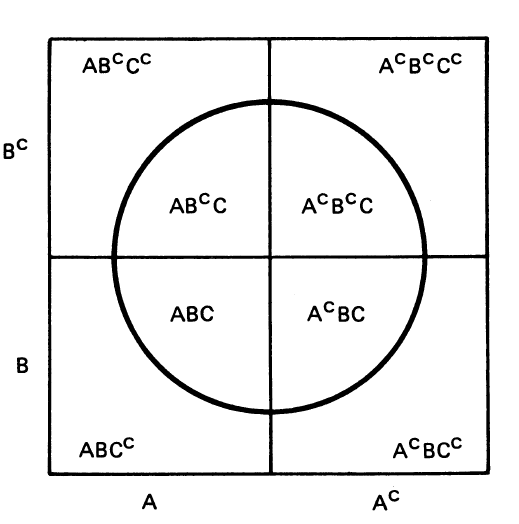
\includegraphics[scale=0.5]{image//Probabilite//1}
\end{wrapfigure}


\chapter{Relations and Operations}
A relation $R$ on $X$ is reflexive if $xRx$ for all $x\in X$,that is,if $R$ contains the $\mathbf{diagonal}$
$$
\bigtriangleup_{X} :=\left \{ (x,x);x\in X \right \}
$$




\chapter{Groups and Homomorphisms}
\section{Cosets}
Let $N$ be a subgroup of G
and $g\in G$.Then $g\odot N$ is the \textbf{left coset} and $N\odot g$ is the \textbf{right coset} of $g\in G$ with respect to $N$ .If we define
$$
g\sim h:\Longleftrightarrow g\in h\odot N
,$$
then $\sim$ is an equivalent relation on $G$:
\textbf{If $\mathbf{g\in h\odot N}$, then there is some $\mathbf{n\in N}$ with $\mathbf{g=h\odot n}$}. Indeed, $\sim$ is reflexive because $e\in N$($g=g\odot e$, 所以$g\sim g$). If $g\in h\odot N$ and $h\in k\odot N$,then
$$
g\in (k\odot N)\odot N=k\odot (N\odot N)=k\odot N
$$




\chapter{Généralité sur espace vectoriel}
\begin{dfn}
        Soient E un ensemble et $\mathbb{K}$ un corps commutatif(ici,$\mathbb{K}=\mathbb{R}$ ou $\mathbb{K}=\mathbb{C}$).On dit que E est un espace vectoriel sur $\mathbb{K}$
(ou bien un $\mathbb{K}$-espace vectoriel)
lorsque E est muni:

-d'une loi de composition interne, notée +,telle que $(E,+)$ soit un group abélien

-d'une loi de omposition externe ,notée $\cdot$, $\cdot$ : $\mathbb{K}\times E \rightarrow E$ vérifiant les propriétés suivantes:

$\bf P1$ $\forall \lambda,\mu \in \mathbb{K},\forall u\in E ,(\lambda+\mu)\cdot u=\lambda\cdot u+\mu\cdot u$

$\bf P2$ $\forall \lambda,\forall u,v\in E ,\lambda\cdot(u+v)=\lambda\cdot u+\lambda\cdot v$


$\bf P3$ $\forall \lambda,\mu \in \mathbb{K},\forall u\in E ,(\lambda\times\mu)\cdot u=\lambda\cdot(\mu\cdot u)$

$\bf P4$ $\forall u\in E ,1_{\mathbb{K}}\cdot u=u$

Les éléments de E sont appelés les vecteurs et les éléments de $\mathbb{K}$ les scalaires
\end{dfn}
\begin{rem}
$(\mathbb{K}^n,+,\cdot)$ est un $\mathbb{K}$-espace vectoriel
\end{rem}
\begin{prp}
        Soit X est un ensemble {\color{red}quelconque} et (F,+,$\cdot$) un $\mathbb{K}$-espace vectoriel.Alors l'ensemble $\mathcal{F}(X,F)$ est un $\mathbb{K}$-espace vectoriel pour les opérations suivantes définies pour tout f,g $\in$ $\mathcal{F}(X,F)$ et $\lambda\in \mathbb{K}$:
\begin{alignat*}{2}
        f\oplus g: X&\rightarrow F&\qquad et \quad \lambda\odot f: X&\rightarrow F\\&x\mapsto f(x)+g(x)
&\quad &x\mapsto \lambda\cdot f(x)
        \end{alignat*}
\end{prp}
\begin{rem}
        Les ensembles $\mathbb{R}^{\mathbb{N}}$,
$\mathbb{R}^{\mathbb{R}}$ et $\mathcal{F}(I,\mathbb{R})$ sont des $\mathbb{R}$-espace vectoriel.Les ensembles $\mathbb{C}^{\mathbb{N}}$,
$\mathbb{C}^{\color{red}\mathbb{R}}$ et $\mathcal{F}(I,\mathbb{C})$ sont des $\mathbb{C}$-espace vectoriel.
\end{rem}
\textbf{之所以给出这些常见的espace vectoriel,是因为我们以后不想再来重复造轮子了,争取一次证明,以后一直用着.}

\begin{rem}
Notez la différence fondamentale dans les règles entre espaces vectoriels et anneaux:

dans un espace vectoriel, $\lambda\cdot u=0\Leftrightarrow  \lambda=0 \quad ou \quad u=0$
\begin{proof}
        $(\lambda\cdot u=0_{E}\Rightarrow \lambda=0_{\mathbb{K}}\quad ou\quad u=0_{E} )\Leftrightarrow(\lambda\cdot u=0_{E}\quad et \quad \lambda\not =0_{\mathbb{K}}\Rightarrow u=0_{E} )$

\textbf{这里用逻辑符号改写,利用同种符号的交换性和否定的改写可以得到这个等价,这样我们就控制了变量。}

        Soient $\lambda$ un scalaire non nul et u un vecteur tels que $\lambda\cdot u=0_{E}$.$\mathbb{K}$ est un corps et $\lambda \not=0_{\mathbb{K}}$ donc $\lambda$ admet un inverse pour la loi $\times$ dans $\mathbb{K}$
Il vient alors:
$$
0_{E}=\lambda^{-1}\cdot 0_{E}=
\lambda^{-1}\cdot(\lambda\cdot u)=(\lambda^{-1}\times\lambda)
\cdot u=1_{\mathbb{K}}\cdot u=u
$$
\end{proof}





dans un anneau,$a\times b=0\not \Rightarrow a=0 \quad ou \quad b=0$
(例子:在($\mathcal{F}(\mathbb{R},\mathbb{R})$,+,$\circ$)这个anneau中定义f和g分别在不同的点不为0,在其他点都为0,则f$\circ$g=0但f$\not$=0且g$\not$=0)
\end{rem}
\begin{dfn}
Soient $u_1,\dots,u_n$ des vecteurs.On appelle combinaison linéaire des vecteurs $u_1,\dots,u_n$ tout
vecteur v sécrivant sous la forme :
$$
v=\sum_{k=1}^{n}\lambda_k\cdot u_k
$$
où $\lambda_1,\dots,\lambda_n$
sont scalaires



\end{dfn}











\begin{dfn}
        Soient E un $\mathbb{K}$-espace vectoriel et F$\subset$E.On dit que F est un sous-$\mathbb{K}$-espace vectoriel de E si:

        (i)$0_{E}\in F$

        (ii)F est stable par combinaisons linéaires
\end{dfn}


\begin{dfn}
        Soient E un espace vectoriel et u un vecteur non nul.On pose alors:
        $$
        \mathbb{K}\cdot u=\left \{ \lambda\cdot u, \lambda\in \mathbb{K} \right \}
        $$
        On dit que $\mathbb{K}\cdot u$ est la droite vectorielle dirigée par u ou que u est un vecteur dircteur de $\mathbb{K}\cdot u$
\end{dfn}
\begin{prp}
        Soit u$\in E\setminus{\{ 0_E\}}$.Alors,    $\mathbb{K}\cdot u$ est un sous-espace vectoriel de E.De plus, tout élément non nul de $\mathbb{K}\cdot u$ est un vecteur directeur de $\mathbb{K}\cdot u$.
\end{prp}






















\chapter{Opération sur les espaces vectoriels}
\section{Intersection et sous-espace engendré par une partie}

\begin{prp}{\bf Intersection}
   Soient E est un $\mathbb{K}$-espace vectoriel et $(F_i)_{i \in I}$ une famille quelconque de sous-espaces vectoriels de E.Alors  $\bigcap_{i \in I}F_{i}$ est un sous-espace vectoriel de E.

\textbf{注意这是一个关于运算的命题,这个运算的被拿出来说的重要性就在这里体现了,也就是子向量空间的交集运算是stable的。}
\end{prp}

\begin{proof}
        On applique les définitions.

        -Pour tout i$\in$I,$F_i$ est un sous-espace vectoriel de E donc:
        $$
        \forall i\in I,0_E\in F_i
        $$
        Ce qui équivaut à $0_E\in\bigcap_{i\in I}F_i$

        -Soient $\lambda,\mu\in \mathbb{K}$ et $u,v \in\bigcap_{i\in I}F_i$.Soit $i \in I$.Puisque $F_i$ est un sous-espace vectoriel de E,$\lambda\cdot u+\mu\cdot v\in F_i$.Ceci étant vrai pour tout $i\in I$,on en déduit que :
$$
\lambda\cdot u+\mu\cdot v\in\bigcap_{i\in I}F_i
$$

Ce qui prouve que $\bigcap_{i\in I}F_i$  est bien un sous-espace vectoriel de E.
\end{proof}










\begin{dfn}{\bf Espace vectoriel engendré par une partie}
Soient E est un $\mathbb{K}$-espace vectoriel et X$\subset$E une partie {\color{red} quelconque} de E.On appelle espace vectoriel
engendré par X,et on note $\mathit{Vect}(X)$
ou $\left \langle X \right \rangle$,l'ensemble défini par :
 \begin{align*}
 \left \langle X \right \rangle = \bigcap_{X\subset F   \atop F sev E}F
 \end{align*}
\end{dfn}

Dans le dessin suivant, on suppose qu'il y a trois sev de E qui contiennent X.(En fait, cette situation ne peut pas se produire en réalité.)
 \begin{figure}[H]
        \centering
        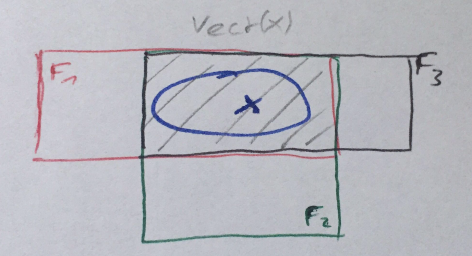
\includegraphics[width=1\textwidth]{image//Operation sur les espaces vectoriels//1}
        \end{figure}

\textbf{注意联系:首先,“叫响名字”:一个是子向量空间的交集运算,一个是从向量空间集E中提取了一个任意子集X来对交集运算中未明的I集合进行抽象的效果定义,即,$I=\left \{i|\quad  X \subset F_i\right \}$, 其实是相当于交集运算中的特例.}

\begin{prp}
        Pour toute partie X$\subset$E,$<X>$ est un sous-espace vectoriel de E et c'est le plus petit sous-espace vextoriel de E(au sens de l'inclusion) qui contient X
\end{prp}
\begin{rem}
        $<\emptyset>=\{0_E\}$
\end{rem}























\section{Somme de sous-espaces vectoriels}
\begin{dfn}{\bf Somme de deux sous-espaces vectoriels }
Soit E un $\mathbb{K}$-espace vectoriel et soient F et G deux sous-espaces vectoriels de E.On définit la somme de F et G, noté $F+G$,
par :
$$F+G=\left \{ u\in E |\quad \exists (x,y)\in F\times G,u=x+y \right \} $$
\end{dfn}
\begin{prp}{\bf Propriété de somme de deux sous-espaces vectoriels}
Avec les hypothèse de la définition , $F+G$ est un sous-espace vectoriel  de contenant F et G, c'est-à-dire que
$$F+G=Vect(F\cup G)$$
\end{prp}
\begin{proof}
        Montrons directement que
        $ F+G=Vect(F\cup G)$,ce qui prouvera également que $F+G$
        est un sous-espace vectoriel de
        E.


        Montrons que $ F+G\subset Vect(F\cup G)$.
        \\
        Soit u $\in F+G$.Par définition , il existe x$\in$F et y$\in$ G tels que u=x+y.On a alors $u=1_\mathbb{K}\cdot x+1_\mathbb{K}\cdot y$ avec x,y $\in$ F$\cup$G et $1_\mathbb{K} \in \mathbb{K}$ donc $u\in \left \langle F\cup G \right \rangle$


        Montrons que $\left \langle F\cup G \right \rangle \subset F+G$
\\
Soit u$\in$	$\left \langle F\cup G \right \rangle$.Il existe $n\in \mathbb{N}, (n)_{0\leq i\leq n}\in
(F+G)^{n+1}$ et $(\lambda_i)_{0\leq i\leq n}\in
\mathbb{K}^{n+1}$ tels que: $u=\sum_{i=0}^{n} \lambda_i x_i$
Posons $I=\left \{ i\in \llbracket 0, n \rrbracket |\quad  x_i\in F \right \}$ et $J= \llbracket 0, n \rrbracket \backslash I$.On a alors
:
$$
u=\sum_{i\in I}\lambda_i x_i\quad+\quad \sum_{j\in J}\lambda_j x_j
$$
Pour tout $i \in I$, $x_i \in F$ et $F$ est un sous-espace vectoriel de $E$ donc: $x=\sum_{i\in I}\lambda_i x_i \in F$.De même, pour tout $j \in J, x_j\in G\backslash F \subset G$
et $G$ est un sous-espace vectoriel
de $E$ donc $y=\sum_{j\in J}\lambda_j x_j \in G
$ .Notez bien que si $I=\emptyset$ ou $J=\emptyset$, le résultat est encore valable puisque $\sum_{i\in \emptyset}\lambda_i x_i=0_E$ qui appartient bien à $F$ et à $G$
.

Ainsi,$u=x+y$ avec $x \in F$  et $x \in G$, c'est-à-dire $u \in F+G$. D'où , la seconde inclusion
\end{proof}

\section{Sommes directes et sous-espaces sectoriels supplémentaires}

\paragraph{Proposition: 直和的等价(具体形式)}
Soient E un $\mathbb{K}$-espace vectoriel et F,G deux sous-espaces vectoriels de E.Alors les propriétés suivantes sont équivalentes:

($i$)F et G sont en somme dircte;

($ii$)Tout éléments u de $F+G$ se décompense de façon unique sous la forme $u-x+y$ avec $x\in F$ et $y\in G$,c'est-à-dire $$\forall u\in F+G, \exists!(x,y)\in F\times G, u=x+y$$
\begin{proof}
        Montrons $(ii)\implies(i)$.
\\
On suppose $(ii)$.Soit $x\in F\cup G$.Alors, par exemple,$(-x)\in G$.Il s'ensuit que $0_E=x+(-x)$ avec $x\in F$ et $(-x)\in G$.Or, on a également $0_E\in F\cup G$ : on peut donc aussi écrire $0_E=0_E+0_E$ avec $(0_E,0_E)\in F\times G$.D'aprês $(ii)$, la décomposition est unique :
ceci implique que $x=0_E$,prouvant ainsi que $F\cup G={0_E}$
\end{proof}
\paragraph{Definition: Supplémentaire}
Soient E un $\mathbb{K}$-espace vectoriel et $F,G$ deux sous-espace vectoriels de E.On dit que $F$ et $G$ sont supplémentaires (ou supplémentaire dans E) si tout vecteur de E peut se décomposer de façon unique en la somme d'un vecteur de F et d'un vecteur de G.Autrement dit $F$ et $G$ sont supplémentaire si:
$$
\forall u\in F+G, \exists!(x,y)\in F\times G, u=x+y
$$

\paragraph{Théorème: Existence du supplémentaire}
Soit E un espace sectoriel et soit F un sous-espace vectoriel de E. Alors F admet au moins un supplémentaire dans E.

\section{Produit cartésien de deux espaces vectoriel}

\chapter{Applications linéaires}
\begin{dfn}{\bf Applications Linéaires}
morphisme
\end{dfn}

\begin{prp}
{\bf Equivalence pour voir si une application  est linéaire}
\textbf{验证线性映射的过程,有一点像验证子向量空间的线性组合stable的过程(区别在于原来是在一个集合内部,现在是两个集合之间),但是因为线性映射的定义的性质中带有$\mathbf{f(0_E)=0_F}$,所以不用看}

\textbf{这个命题还是比较有意思的,有助于理解线性映射的定义和外延.注意如何在未知是线性映射的情况下要重新证明$\mathbf{f(0_E)=0_F}$}

$\mathbf{f:\mathbb{R}^2\longrightarrow \mathbb{R}^2,\quad (x,y)\longmapsto (2x,x+y)} $
\textbf{比较抽象的线性映射}

否定一个线性映射可以用$f(0_E)\neq 0_F$来判断
\end{prp}

\paragraph{Définition: forme linéaire}





\subsection{Restriction et recollement}
\begin{thm}{\bf Théorème de recollement}  Soient E,F deux $\mathbb{K}$-espaces vectoriels et G,H deux sous-espaces vectoriels supplémentaire dan E.Alors l'application:
\begin{align*}
\phi:\mathcal{L}(E,F)\rightarrow \mathcal{L}(G,F)\times \mathcal{L}(H,F)\\
f\mapsto (f|_{G},f|_{H})
\end{align*}
est un isomorphisme de $\mathbb{K}$-espaces vectoriels.En clair ,la connaissance d'une application linéaire sur deux sous-espaces  vectoriels supplémentaire détermine l'application linéaire de façon unique.
\end{thm}
\begin{proof}
        \begin{itemize}


\item Tout d'abord,d'après ce qui précède ,$\mathcal{L}(E,F),\mathcal{L}(G,F),\mathcal{L}(H,F)$ sont des $\mathbb{K}$-espace vectoriel.Par suite,$\mathcal{L}(G,F)\times\mathcal{L}(H,F)$ est aussi un
$\mathbb{K}$-espace vectoriel.
\item Ensuite,d'après la proposition précédente,si $f\in\mathcal{L}(E,F)$,alors $f_{|G}\in\mathcal{L}(G,F)$
et $f_{|H}\in\mathcal{L}(H,F)$.Par conséquent,$\phi$ est bien définie.
\item Par ailleurs, il est clair que pour toutes $f,g\in
\mathcal{L}(E,F)$,pour tout $\lambda,\mu\in\mathbb{K}$,et pour tout sous-espace vectoriel A de E,$(\lambda\cdot f+\mu\cdot g)
_{|A}=\lambda\cdot f_{|A}+\mu\cdot g_{|A}$.
Par suite,$\phi$ est linéaire.
\item Montrons enfin que $\phi$ est bijective.

-Injectivité

Soit $f\in ker\phi$.Montrons que $f=0$.Par définition de $\phi$,$f_{|G}=0$ et $f_{|H}=0$.Soit alors $x\in E$
Puisque G et H sont supplémentaires dans E,il existe un unique couple (a,b)$\in G\times H$ tel que $x=a+b$.On a alors :

\begin{alignat*}{5}
    f(x)&=f(a+b)\\
    &=f(a)+f(b)\\
    &=f_{|G}(a)+f_{|H}(b)\\
    &=0+0\\
    &=0
\end{alignat*}
Par conséquant,pour tout $x\in E,f(x)=0$,c'est-à-dire $f=0$(application nulle) et $ker\phi=\{0\}$,c'est-à-dire $\phi$ est injective.

-Surjectivité

Soient g$\in \mathcal{L}(G,F)$ et h$\in \mathcal{L}(H,F)$,Montrons qu'il existe $f\in \mathcal{L}(E,F)$ telle que
$f_{|G}\in\mathcal{L}(G,F)$
et $f_{|H}\in\mathcal{L}(H,F)$.

Soit $x\in E$:il exist un unique couple $(a,b)\in G\times H$ tel que $x=a+b$.On pose alors $f(x)=g(a)+h(b)$.Ceci définit bien une application $f$ de E dans F puisque le couple (a,b)
est unique.Montrons alors que
$f$ convient.
\begin{itemize}
 \item Si $x\in G$,alors par unicité du couple $(a,b)\in G\times H$ tel que $x=a+b$,on a $a=x$ et $b=0$.Alors,$f(x)=g(a)+h(b)=g(x)+h(0)=g(x)+0=g(x)$.Par suite,$f_{|G}=g$.
 \item De la même façon,on montre que $f_{|H}=h$.
 \item Montrons enfin que $f\in\mathcal{L}(E,F)$.

 Soient $x,x'\in E$ et $\lambda \in \mathbb{K}$.
 Il existe alors un unique couple $(a,b)\in G\times H$ et un unique couple $(a,b)\in G\times H$ tels que $x=a+b$ et $x'=a'+b'$.On a alors $\lambda \cdot x+x'=(\lambda\cdot a+a')+(\lambda\cdot b+b')$.G et H étant des sous-espaces vectoriels de E,$ (\lambda\cdot a+a',\lambda\cdot b+b')\in G\times H$,Par suite,
 \begin{alignat*}{4}
 f(\lambda\cdot x+x')&=g(\lambda\cdot a+a')+h(\lambda\cdot b+b')\\
 &=\lambda \cdot g(a)+g(a')+\lambda\cdot h(b)+h(b')\\
 &=\lambda\cdot(g(a)+h(b))+g(a')+h(b')\\
 &=\lambda\cdot f(x)+f(x')
 \end{alignat*}
 Ce qui prouve que $f$ est une application linéaire.
\end{itemize}
\end{itemize}
Ainsi,on a montre que pour tout $(g,h)\in \mathcal{L}(G,F)\times \mathcal{L}(H,F)$ qu'il existe $f\in \mathcal{L}(E,F)$ telle que
$f_{|G}\in\mathcal{L}(G,F)$
et $f_{|H}\in\mathcal{L}(H,F)$,c'est-à-dire $\phi(f)=(g,h)$.Par conséquant,$\phi$ est surjective.

\end{proof}
\chapter{Integration}
We now turn to integration, which we develop as the ‘area under the curve’. We establish the existence and properties of the Riemann integral; this is an integral whose development is quite straightforward, and which is good for many of the needs of analysis. It has some shortcomings: it can only be applied to a restricted class of functions, and it is not easy to obtain good results about limits of integrals. For this, a more sophisticated(复杂的) integral, the Lebesgue integral, is needed.

As with all theories of integration, we proceed by approximation. To
begin with, we restrict attention to bounded real-valued functions on
a finite interval $[a, b].$ The easiest functions to start with are
the step functions —— functions which take constant values $v_j$ on a
finite set $\left\{I_j : 1 \le j \le k\right\}$ of disjoint
sub-intervals of $[a, b].$ The graph of such a function is a bar
graph, and we define the elementary integral of such a function to be
$\sum^k_{j=1} v_jl(I_j),$ where $l(I_j)$ is the length of the interval
$I_j.$ Note that $v_j$ can be positive or negative, so that the
integral can take positive and negative values. The idea of the
Riemann integral of a function $f$ is to approximate $f$ from above
and below by step functions. If the integrals of the approximations
from above and from below approach a common limit, then we take this
limit to be the Riemann integral of $f.$ In order to carry out this
programme, we need to set up the appropriate machinery. A
{\bf{dissection}} $D$ of $[a, b]$ is a {\bf finite subset} of $[a, b]$ which contains both $a$ and $b.$ We arrange the elements of $D,$ the points of dissection of $D,$ in increasing order: $a = x_0 < x_1 < \cdots < x_k = b.$ The dissection splits $[a, b]$ into $k$ disjoint intervals $I_1,\cdots I_k.$ We need to decide what to do with the endpoints; we adopt the convention that $I_1 = [x_0, x_1]$ and that $I_j = (x_{j−1}, x_j ]$ for $2 \le j<k.$
We order the dissections of $[a, b]$ by inclusion: we say that $D_2$ {\bf{refines}} $D_1$ if $D_1 \subset D_2,$ and write $D_1 \le D_2.$ This is a partial order on the set $\Delta$ of all dissections of $[a, b],$ and $\Delta$ is a lattice: $D_1\vee D_2 = D_1 \cup D_2$ and $D_1 \wedge D_2 = D_1 \cap D_2.$ $\Delta$ has a least element $\left\{a, b\right\},$ but has no greatest element.
Suppose that $D$ is a dissection, with intervals $I_1,\cdots,I_k.$ We denote the indicator function of $I_j$ by $\chi_j$ : $\chi_j (x) = 1$ if $x \in I_j,$ and $\chi_j (x) = 0$ otherwise. Similarly, we write $\chi_{[a,b]}$ for the indicator function of $[a, b].$ We denote the linear span of $\left\{\chi_j : 1 \le j \le k\right\}$ by $E_D;$ thus a function $f \in E_D$ is of the form $f =\sum^k _{j=1} v_j\chi_j ,$ where $v_1,\cdots,v_k$ are real numbers. The elements of $E_D$ are the step functions on $[a, b]$ whose points of discontinuity are contained in $D;$ note that, according to our convention, step functions are continuous on the left. $E_D$ is a $k$-dimensional vector space of functions. If $D_2$ refines $D_1,$ then $E_{D_1} \subset E_{D_2},$ and so the set of spaces $\left\{E_D : D \in \Delta\right\}$ also forms a lattice:
$$
\begin{aligned}
  E_{D_{1}} & \wedge E_{D_{2}}=E_{D_{1}} \cap E_{D_{2}}=E_{D_{1} \wedge D_{2}}
\end{aligned}
$$
and
$$
\begin{aligned}
 E_{D_{1}} \vee E_{D_{2}} &=\operatorname{span}\left(E_{D_{1}} \cup E_{D_{2}}\right)=E_{D_{1} \vee D_{2}}
\end{aligned}
$$
The union $E_{\Delta}=\cup\left\{E_{D}: D \in \Delta\right\}$ is the infinite-dimensional vector space of all (left-continuous) step functions.
We now wish to define the elementary integral of a step function $f .$ If $f=\sum_{j=1}^{k} v_{j} \chi_{j},$ we want to define $\int_{a}^{b} f(x) d x$ to be $\sum_{j=1}^{k} v_{j} l\left(I_{j}\right),$ where $l\left(I_{j}\right)=x_{j}-x_{j-1}$ is the length of $I_{j} .$ But the representation is not unique, and we need to show that the integral is well-defined.
\begin{prp}
  Suppose that $D$ and $D'$ are dissections of $[a, b],$ and that $f \in E_D\cap E_D' ,$ with representations $f =\sum^k_{j=1} v_j\chi_j$ and $f =\sum^{k'}_{j=1} v'_j\chi'_j .$ Then $$\sum^k_{j=1}v_jl(I_j)=\sum^{k'}_{j=1} v'_j l(I'_j).$$
\end{prp}
\begin{proof} We use the lattice property of $\Delta.$ Let $D'' = D \cup D'.$ Let $D = \left\{x_0,\cdots,x_k\right\}$ and $D'' = \left\{x''_0,\cdots,x''_{k''}\right\}.$ Then there exist $0 = r_0 < r_1 < \cdots < r_k = k''$ such that $x_j = x''_{r_j}$ for $0 \le j \le k.$ Thus $$l(I_j) =\sum^{r_j}_{r=r_{j−1}+1} l(I''_r).$$ 注意区间是按后一个点的序号算,这里求和的$r$是按1到$k''$的序走,不是按$r_{k}$的角标序(1到$k$)走.We can write $f =\sum^{k''}_{r=1} v''_r\chi''_r,$ where $v_j = v''_r$ for $r_{j−1} < r \le r_j.$ Consequently, $$\sum^k_{j=1}v_j l(I_j) = \sum^k_{j=1} \left( \sum^{r_j}_{r=r_{j−1}+1} v''_r l(I''_r )\right) = \sum^{k''}_{r=1} v''_r l(I''_r).$$
Similarly, $\sum^{k'}_{j=1}v'_j l(I'_j)=\sum^{k''}_{r=1} v''_r l(I''_r)$, so that $$\sum^k_{j=1}v_jl(I_j)=\sum^{k'}_{j=1} v'_j l(I'_j).$$
We can therefore define the elementary integral as $$\int_{a}^{b} f(x) d x=  \sum^k_{j=1}v_jl(I_j).$$
\end{proof}
\begin{rem}
A partially ordered set $(A, \le)$ is called a {\bf{lattice}} if
whenever $a$ and $b$ are elements of $A$ then the set $\left\{a,
  b\right\}$ has an infimum, denoted by $a\wedge b,$ and a supremum,
denoted by $a \vee b.$
\end{rem}
\section{Upper and lower Riemann integrals}
We now consider a bounded function f on [a, b], with $m \le f(x) \le M$ for all
$x \in [a, b].$  We try to integrate it by approximating from above and below by
step functions. Let
$$U_f = \left\{g : g \in E_{\Delta}\text{ and }g \ge f\right\}$$
be the set of step functions which are greater than or equal to $f$. $U_f$ is
non-empty, since $M_{\chi_{[a,b]}} \in U_f$. If $g \in U_f, g \ge m_{\chi_{[a,b]}}$, and so
$\int_{a}^{b}g(x) dx \ge m(b-a)$.Thus the set $\left\{\int^b_a g(x) dx : g \in U_f\right\}$ is bounded below. We define
the {\bf upper Riemann integral} of f to be
$$
\overline{\int^b_a}f(x)d x=\inf\left\{\int^b_a g(x) dx : g \in U_f\right\}
$$
很诡异的定义: 先定义f的“上阶分(阶梯分划)集”,然后给“上阶分集”的定积分集取$\inf$,也就是在
“上阶分集”的定积分集的下界中找一个最大值,即:{\bf 上下上}.上下不在一个范畴内,一
个是阶梯函数集,一个是定积分集.

Similarly we set
$$L_f = \left\{h : h \in E_{\Delta}\text{ and }h \le f\right\}$$
and define the {\bf lower Riemann integral} of f to be
$$
\underline{\int^b_a}f(x)d x=\sup\left\{\int^b_a h(x) dx : h \in L_f\right\}
$$
\begin{prp}
Suppose that $f$ is a bounded function on $[a, b] .$ Then $\underline{\int_{a}^{b}} f(x) d x \leq \overline{\int_{a}^{b}} f(x) d x$
\end{prp}
\begin{proof}
$\quad$ If $h \in L_{f}$ and $g \in U_{f}$ then $h \leq f \leq g,$ so that
$$
\int_{a}^{b} h(x) d x \leq \int_{a}^{b} g(x) d x
$$
Taking the supremum over $L_{f},$ we see that
$$
\underline{\int_{a}^{b}} f(x) d x \leq \int_{a}^{b} g(x) d x,
$$
so that, taking the infimum over $U_{f}$,
$$
\underline{\int_{a}^{b}} f(x) d x \leq \inf \left\{\int_{a}^{b} g(x) d x: g \in U_{f}\right\}=\overline{\int_{a}^{b}} f(x) d x
$$
\end{proof}
Suppose that D is a dissection, with intervals $I_1, \cdots , I_k$, and that f is
a bounded function on [a, b]. Let $M(I_j) =\sup\left\{f(x) : x \in I_j\right\}$, and let
$M_D(f) = \sum^k_{j=1} M_j\chi_j$. Then $M_D(f)$ is the least element of $E_D \cap U_f =\left\{g \in
E_D, g \ge f\right\}$.这时候又对“上阶分集”中的函数取了最小值,但这个最小
值函数又是在对函数值的上集取了最小值的基础上构建的. We set
$$S_D = S_D(f) =\sum^k_{j=1}M(I_j)l(I_j) =\int^b_aM_D(f)(x) d x.$$
这个地方就是难点交汇处,我们要找的是所有“上阶分集”中函数的积分集的下界的最大值,我
们构造了一个对特定划分的“上阶分集”中的函数的最小值,现在需要建立它们之间的联系。
Then $$S_D = \inf\left\{\int^b_a g(x) dx : g \in U_f \cap E_D\right\},$$
对应关系:“上阶分集”中函数的积分集的下界的最大值=“上阶分集”中的最
小值函数的积分.这里简化就是:“下界的最大值”=最小值.这是成立的.因为最小值
是实打实存在的,这是阶梯函数的特殊性,可以类比于整数相对于实数的特殊性.顺
便吐槽一下,这里的困惑全部来源于对$\sup,$$\inf,$$\min,$和$\max$不加证
明的使用,可见法国人的严谨是有必要的,步步为营最后反而赢得时间,
so that
$$\begin{aligned}
\overline{\int^b_a}f(x) dx &=\inf\left\{\inf\left\{
\int^b_ag(x) dx : g \in U_f \cap E_D\right\} : D \in \Delta\right\}\\
&=\inf\left\{S_D : D \in \Delta\right\}.
\end{aligned}$$
Similarly, we define $m(I_j) =\inf\left\{f(x) : x \in I_j\right\}$ and
$m_D(f) = \sum^k_{j=1} m_j(I_j)\chi_j$
and set $$s_D = s_D(f) =\sum^k_{j=1}m(I_j)l(I_j) =\int^b_am_D(f)(x) d x.$$
Then $$s_D = \sup\left\{\sup\int^b_a h(x) dx : h \in L_f \cap E_D\right\},$$ so that
$$\begin{aligned}
\underline{\int^b_a}f(x) dx &=\sup\left\{\sup\left\{
\int^b_ah(x) dx : h \in L_f \cap E_D\right\} : D \in \Delta\right\}\\
&=\sup\left\{s_D : D \in \Delta\right\}.
\end{aligned}$$
\begin{figure}[H]
  \centering
  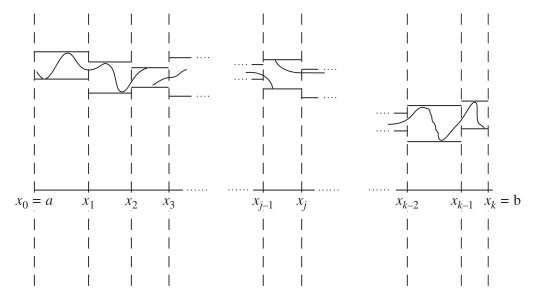
\includegraphics[width=0.8\linewidth]{image//Integration//1}
  \caption{Upper and lower sums $S_D$ and $s_D$.}
\end{figure}
Note that if $D^{\prime}$ refines D then $S_{D^{\prime}} \le S_D$ and $s_{D^{\prime}} \ge s_D$.

In fact, we do not need to consider all the dissections to determine the
upper and lower Riemann integrals. If D is a dissection, with intervals
$I_1, \cdots, I_k$, we define the {\bf mesh size} $\delta(D)$ to be $\max\left\{l(I_j) : 1 \le j \le k\right\}$.

\begin{thm}
Suppose that $(D_r)^{\infty}_{r=1}$ is a sequence of dissections of [a, b],
and that $\delta(D_r) \to 0$ as $r \to \infty$. If f is a bounded function on [a, b] then
$S_{D_r}(f) \to\overline{\int^b_a} f(x) d x$ as $r\to\infty$.
\end{thm}
\begin{proof}
Suppose that $\epsilon > 0$. Then there exists a dissection D of [a, b],
with points of dissection $a = x_0 < x_1 < \cdots < x_k = b$ such that
$S_D <\int^b_a f(x) dx + \epsilon/2.$ The idea of the proof is to choose r large enough so
that the set D is contained in a set of intervals of $D_r$ of small
total length.(这里的D是分点的集合,但我们要求的是$D_r$划分的小区间(每个
小区间的长度都很短)要包含组成D的分点,可以说又一次有点跳脱维度) Let
$\eta = \frac{\epsilon}{2(k + 1)(M − m + 1)}$. There exists $r_0$ such that $\delta(D_r) < \eta$ for $r \ge r_0$.
Suppose that $r \geq r_{0} .$ Let $D^{\prime}=D \vee D_{r} .$ Then $S_{D^{\prime}} \leq S_{D} .$ Let $\left\{J_{1}, \ldots, J_{q}\right\}$
be the intervals of the dissection $D_{r},$ and let $K_{1}, \ldots,
K_{s}$ be the intervals of the dissection $D^{\prime} .$ We divide
$\{1, \ldots, q\}$ into two disjoint subsets. Let $p \in B$ if $J_{p}$
contains one or more elements of $D,$ and let $p \in G$
otherwise. $(B$ is the set of bad indices, and $G$ is the set of good
indices.) Then $|B| \leq k+1$. If $p \in B,$ then $J_{p}$ is the
disjoint union $\cup_{r \in S_{p}} K_{r}$(所有此$J_p$旗下包含的D的
端点把此$J_P$二次分化后,对应到$D^{\prime}$中划分出区间的序号) of finitely many of
intervals in $D^{\prime} .$  Since $m \le f(x) \le M,$
$$M l\left(J_{p}\right) \geq M\left(J_{p}\right) l\left(J_{p}\right) \geq \sum_{r \in S_{p}} M\left(K_{r}\right) l\left(K_{r}\right) \geq m \sum_{r \in S_{p}} l\left(K_{r}\right)=m l\left(J_{p}\right) .
$$
If $p \in G,$ then $J_{p}=K_{r}$ for some $r \in\{1, \ldots, s\},$ so that $M\left(J_{p}\right)=M\left(K_{r}\right)$ Thus
$$
\begin{aligned}
S_{D_{r}}-S_{D^{\prime}} &\left.=\sum_{p \in
    B} \left(M_{p}l\left(J_{p}\right)-\sum_{r \in S_{p}}
    M\left(K_{r}\right) l(K_{r}) \right)\right. \\
& \leq \sum_{p \in B}(M-m) l\left(J_{p}\right) \leq(M-m)(k+1) \delta\left(D_{r}\right)<\epsilon / 2
\end{aligned}
$$
Consequently, if $r \geq r_{0}$ then
$$
\int_{a}^{b} f(x) d x \leq S_{D_{r}} \leq S_{D^{\prime}}+\epsilon / 2 \leq S_{D}+\epsilon / 2<\int_{a}^{b} f(x) d x+\epsilon
$$
so that $S_{D_{r}} \rightarrow \overline{\int_{a}^{b}} f(x) d x$ as $r
\rightarrow \infty$


\end{proof}


\end{document}
